Để đơn giản, trong bài toán này, ta sẽ sử dụng hệ tọa độ Gauss với $4 \pi \varepsilon_0 = 1$.
\begin{enumerate}
    \item 
    \begin{enumerate}[label=\textbf{\alph*,}]\itemsep0em
        \item Điện thế tại điểm $(\rho,z)$ gây ra bởi sợi dây:
    \begin{equation} \label{eq1_ellipsoid_conductor}
        \phi = \int_{-L}^{L} \dfrac{1}{\sqrt{\rho^2+(z-l)^2}} \dfrac{Q}{2L} dl = \dfrac{Q}{2L} \left[ \sinh^{-1}\left(\dfrac{z+L}{\rho}\right)-\sinh^{-1}\left(\dfrac{z-L}{\rho}\right) \right].
    \end{equation}
    \item 
    Từ đây, ta thu được phương trình mặt đẳng thế hình Ellipse tròn xoay $ \left( \dfrac{z}{a} \right)^2 + \left( \dfrac{\rho}{b} \right)^2 = 1$ với hai bán trục của Ellipse lần lượt là $a = L \coth \left( \dfrac{L \phi}{Q} \right)$ và $b = \dfrac{L}{ \sinh \left( \dfrac{L \phi}{Q} \right)}$. \footnote{Xem thêm các biến đổi chi tiết ở cuối lời giải.} \\
    \end{enumerate}
    \item
    \begin{enumerate}[label=\textbf{\alph*,}]\itemsep0em
        \item Điện trường do một thanh thẳng có độ dài $2L=2\sqrt{a^2-b^2}$ tích điện $Q$ phân bố đều gây ra hoàn toàn mô tả chính xác điện trường vùng không gian bên ngoài ellipsoid dẫn trong bài toán. Thật vậy, nó thỏa mãn toàn bộ các phương trình về điện trường tĩnh, cũng như thỏa mãn điều kiện biên về mặt đẳng thế của vật dẫn. Thay $L=\sqrt{a^2-b^2}$ vào kết quả phần \textbf{1.} ta tìm được điện dung của ellipsoid dẫn
        \begin{equation} \label{eq2_ellipsoid_conductor}
            C=\dfrac{Q}{\phi} = \dfrac{\sqrt{a^2-b^2}}{ \cosh^{-1} \left( \dfrac{a}{b} \right)}.
        \end{equation}
        \item Mật độ điện mặt của vật dẫn bằng với độ lớn của vector cảm ứng điện trường tại bề mặt, hay cũng chính bằng vector cường độ điện trường trong trường hợp này
        \begin{equation} \label{eq3_ellipsoid_conductor}
            \sigma = \dfrac{1}{4\pi} \left| \Vec{E} \right| = \dfrac{1}{4\pi} \left| - \nabla \phi \right| = \dfrac{Q}{4 \pi ab^2} \left( \dfrac{z^2}{a^4} + \dfrac{\rho^2}{b^4} \right)^{-1}.
        \end{equation}
    \end{enumerate}
\end{enumerate}

\textbf{ \textit{Các bước biến đổi chi tiết cho phần 1b.}}
    \begin{align*}
        & \phi = \dfrac{Q}{2L} \left[ \sinh^{-1}\left(\dfrac{z+L}{\rho}\right)-\sinh^{-1}\left(\dfrac{z-L}{\rho}\right) \right]. \\
        & \Rightarrow \sinh^{-1}\left(\dfrac{z-L}{\rho}\right) + \dfrac{2L\phi}{Q}
        = \sinh^{-1}\left(\dfrac{L+z}{\rho}\right) \\
        & \Rightarrow \sinh\left(\dfrac{2L\phi}{Q}\right)\sqrt{1+\left(\dfrac{z-L}{\rho}\right)^2}+\cosh\left(\dfrac{2L\phi}{Q}\right)\dfrac{z-L}{\rho} = \dfrac{z+L}{\rho} \\
        & \Rightarrow \dfrac{z\left[1-\cosh\left(\dfrac{2L\phi}{Q}\right)\right]+L\left[1+\cosh\left(\dfrac{2L\phi}{Q}\right)\right]}{\rho} = \sinh\left(\dfrac{2L\phi}{Q}\right)\sqrt{1+\left(\dfrac{z-L}{\rho}\right)^2}  \\
        & \Rightarrow \dfrac{\rho^2\sinh^2\left(\dfrac{2L\phi}{Q}\right)}{2L^2\left[1+\cosh\left(\dfrac{2L\phi}{Q}\right)\right]}+\dfrac{z^2\left[\cosh\left(\dfrac{2L\phi}{Q}\right)-1\right]}{L^2\left[\cosh\left(\dfrac{2L\phi}{Q}\right)+1\right]} = 1 \\
        & \Rightarrow \dfrac{\rho^2}{L^2}\sinh^2\left(\dfrac{L\phi}{Q}\right)+\dfrac{z^2}{L^2}\tanh^2\left(\dfrac{L\phi}{Q}\right) = 1.
    \end{align*}

\textbf{ \textit{Một số cách làm khác để chứng minh mặt đẳng thế là ellipsoid:}}

\textit{+Cách 1:} Định nghĩa quỹ tích

Từ hàm điện thế vô hướng xác định được ở phần 1, ta có thể viết lại:

\begin{equation} \label{eq4_ellipsoid_conductor}
    \phi = \dfrac{Q}{2L} \ln \left[ \dfrac{\sqrt{(L+z)^2 +\rho^2} + \sqrt{(L-z)^2 + \rho^2} + 2L}{\sqrt{(L+z)^2 + \rho^2} + \sqrt{(L-z)^2 + \rho^2} - 2L} \right].
\end{equation}
Tức là mặt đẳng thế thỏa mãn phương trình mặt:
\begin{equation} \label{eq5_ellipsoid_conductor}
    \sqrt{(L+z)^2 + \rho^2} + \sqrt{(L-z)^2 + \rho^2} = 2 L \coth \left( \dfrac{L \phi}{Q} \right).
\end{equation}
Đây là quỹ tích của mặt ellipsoid có hai tiêu điểm nằng tại hai đầu dây tích điện và bán trục lớn $a= L \coth \left( \dfrac{L \phi}{Q} \right)$. Tâm sai của ellipse này theo đó là $e=\coth \left( \dfrac{L \phi}{Q} \right)$, tức là bán trục nhỏ $b= a \sqrt{1-e^2} = \dfrac{L}{ \sinh \left( \dfrac{L \phi}{Q} \right)}$.

\textit{+Cách 2:} Sử dụng tính chất phản chiếu của ellipse: \\
Xét một điểm $M$ bất kỳ trong không gian nằm cách đường thẳng chứa dây điện tích một đoạn $\rho$, $N$ là một điểm nằm trên dây tích điện $AB$ sao cho $MN$ là tia phân giác $\angle AMB$.

\begin{center}


\tikzset{every picture/.style={line width=0.75pt}} %set default line width to 0.75pt        

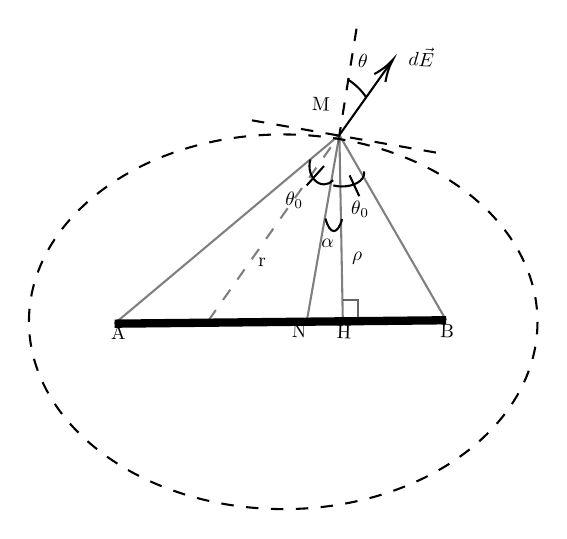
\begin{tikzpicture}[x=0.75pt,y=0.75pt,yscale=-1,xscale=1]
%uncomment if require: \path (0,329); %set diagram left start at 0, and has height of 329

%Shape: Boxed Line [id:dp18134862073246527] 
\draw [color={rgb, 255:red, 0; green, 0; blue, 0 }  ,draw opacity=0.5 ]   (157.09,187.11) -- (265.42,96.21) ;
%Shape: Boxed Line [id:dp12099064274809379] 
\draw [color={rgb, 255:red, 0; green, 0; blue, 0 }  ,draw opacity=0.5 ]   (265.42,96.21) -- (316.85,185.46) ;
%Shape: Boxed Line [id:dp20049333748183473] 
\draw [color={rgb, 255:red, 0; green, 0; blue, 0 }  ,draw opacity=0.5 ]   (265.42,96.21) -- (249.65,186.26) ;
%Shape: Boxed Line [id:dp17865478996636575] 
\draw [color={rgb, 255:red, 0; green, 0; blue, 0 }  ,draw opacity=1 ][line width=3]    (157.09,187.11) -- (316.85,185.46) ;
%Straight Lines [id:da8125496874210176] 
\draw [color={rgb, 255:red, 0; green, 0; blue, 0 }  ,draw opacity=0.5 ] [dash pattern={on 4.5pt off 4.5pt}]  (202.45,185.46) -- (265.42,96.21) ;
%Straight Lines [id:da6002158392672337] 
\draw    (265.42,96.21) -- (290.1,61.49) ;
\draw [shift={(291.25,59.86)}, rotate = 125.4] [color={rgb, 255:red, 0; green, 0; blue, 0 }  ][line width=0.75]    (10.93,-3.29) .. controls (6.95,-1.4) and (3.31,-0.3) .. (0,0) .. controls (3.31,0.3) and (6.95,1.4) .. (10.93,3.29)   ;
%Straight Lines [id:da8906366441589808] 
\draw  [dash pattern={on 4.5pt off 4.5pt}]  (273.67,45) -- (265.42,96.21) ;
%Shape: Boxed Line [id:dp4280899838487169] 
\draw  [dash pattern={on 4.5pt off 4.5pt}]  (311.93,104.67) -- (221.88,88.9) ;
%Shape: Arc [id:dp1052035780036713] 
\draw  [draw opacity=0] (269.36,69.39) .. controls (272.88,71.58) and (275.96,74.51) .. (278.34,78.03) -- (253.48,94.84) -- cycle ; \draw   (269.36,69.39) .. controls (272.88,71.58) and (275.96,74.51) .. (278.34,78.03) ;  
%Shape: Boxed Line [id:dp6660278877118841] 
\draw [color={rgb, 255:red, 0; green, 0; blue, 0 }  ,draw opacity=0.5 ]   (265.42,96.21) -- (267.05,184.66) ;
%Shape: Ellipse [id:dp9767305005316875] 
\draw  [dash pattern={on 4.5pt off 4.5pt}] (115.85,185.92) .. controls (115.96,136.07) and (170.9,95.78) .. (238.56,95.94) .. controls (306.22,96.09) and (360.98,136.62) .. (360.86,186.47) .. controls (360.75,236.32) and (305.81,276.6) .. (238.15,276.45) .. controls (170.49,276.3) and (115.74,235.76) .. (115.85,185.92) -- cycle ;
%Shape: Arc [id:dp6554054937575013] 
\draw  [draw opacity=0] (262.42,118.01) .. controls (261.22,119.26) and (259.68,120) .. (258,120) .. controls (254.13,120) and (251,116.05) .. (251,111.17) .. controls (251,110.07) and (251.16,109.02) .. (251.45,108.06) -- (258,111.17) -- cycle ; \draw   (262.42,118.01) .. controls (261.22,119.26) and (259.68,120) .. (258,120) .. controls (254.13,120) and (251,116.05) .. (251,111.17) .. controls (251,110.07) and (251.16,109.02) .. (251.45,108.06) ;  
%Shape: Arc [id:dp556244560380825] 
\draw  [draw opacity=0] (277.25,113.73) .. controls (277.32,114.03) and (277.35,114.33) .. (277.35,114.64) .. controls (277.35,118.16) and (272.58,121.01) .. (266.69,121.01) .. controls (265.2,121.01) and (263.79,120.83) .. (262.5,120.5) -- (266.69,114.64) -- cycle ; \draw   (277.25,113.73) .. controls (277.32,114.03) and (277.35,114.33) .. (277.35,114.64) .. controls (277.35,118.16) and (272.58,121.01) .. (266.69,121.01) .. controls (265.2,121.01) and (263.79,120.83) .. (262.5,120.5) ;  
%Shape: Right Angle [id:dp627154132195284] 
\draw  [color={rgb, 255:red, 0; green, 0; blue, 0 }  ,draw opacity=0.6 ] (267.05,175.66) -- (274.55,175.66) -- (274.55,184.66) ;
%Shape: Arc [id:dp2502467223266438] 
\draw  [draw opacity=0] (266.73,136.68) .. controls (265.77,140.24) and (264.34,142.5) .. (262.75,142.5) .. controls (261.13,142.5) and (259.68,140.15) .. (258.71,136.46) -- (262.75,125.75) -- cycle ; \draw   (266.73,136.68) .. controls (265.77,140.24) and (264.34,142.5) .. (262.75,142.5) .. controls (261.13,142.5) and (259.68,140.15) .. (258.71,136.46) ;  
%Straight Lines [id:da42998185574073755] 
\draw    (258,111.17) -- (249.67,120.5) ;
%Straight Lines [id:da6176729001517964] 
\draw    (270.33,115.67) -- (275,125.67) ;

% Text Node
\draw (251.36,76.74) node [anchor=north west][inner sep=0.75pt]  [rotate=-2,xscale=0.7,yscale=0.7] [align=left] {M};
% Text Node
\draw (154.39,187.16) node [anchor=north west][inner sep=0.75pt]  [xscale=0.7,yscale=0.7] [align=left] {A};
% Text Node
\draw (313.19,186.29) node [anchor=north west][inner sep=0.75pt]  [rotate=-2,xscale=0.7,yscale=0.7] [align=left] {B};
% Text Node
\draw (241.69,186.1) node [anchor=north west][inner sep=0.75pt]  [rotate=-2,xscale=0.7,yscale=0.7] [align=left] {N};
% Text Node
\draw (273.56,56.07) node [anchor=north west][inner sep=0.75pt]  [rotate=-2,xscale=0.7,yscale=0.7] [align=left] {$\displaystyle \theta $};
% Text Node
\draw (297.98,52.8) node [anchor=north west][inner sep=0.75pt]  [rotate=-2,xscale=0.7,yscale=0.7] [align=left] {$\displaystyle d\vec{E}$};
% Text Node
\draw (263.36,186.94) node [anchor=north west][inner sep=0.75pt]  [rotate=-2,xscale=0.7,yscale=0.7] [align=left] {H};
% Text Node
\draw (225.35,154.47) node [anchor=north west][inner sep=0.75pt]  [rotate=-2,xscale=0.7,yscale=0.7] [align=left] {r};
% Text Node
\draw (238.33,122.5) node [anchor=north west][inner sep=0.75pt]  [xscale=0.7,yscale=0.7] [align=left] {$\displaystyle \theta _{0}$};
% Text Node
\draw (270.05,127.04) node [anchor=north west][inner sep=0.75pt]  [xscale=0.7,yscale=0.7] [align=left] {$\displaystyle \theta _{0}$};
% Text Node
\draw (270.5,151.5) node [anchor=north west][inner sep=0.75pt]  [xscale=0.7,yscale=0.7] [align=left] {$\displaystyle \rho $};
% Text Node
\draw (255.67,145.33) node [anchor=north west][inner sep=0.75pt]  [xscale=0.7,yscale=0.7] [align=left] {$\displaystyle \alpha $};


\end{tikzpicture}
\end{center}

% \begin{center}
% \begin{tikzpicture}
%     \draw[dashed, thick] (0,0) ellipse (4 and 2);
%     \draw[ultra thick] (-2,0) to (2,0);
%     \draw (-2,0) to (1.5,1.85) to (2,0);
%     \draw (1.5,1.85) to (0.6,0);
%     \draw[dashed] (1.5,1.85) to (1.5,0);
%     \draw (1.5,0.2) to (1.3,0.2) to (1.3,0);
% \end{tikzpicture}
% \end{center}

Với $\theta$ là góc hợp bởi đường nối từ một điểm trên dây và $MN$, vi phân độ dài một đoạn dây tích điện $dl=\rho d\theta /[\cos^2(\theta+\alpha)]$.
Ta tính điện trường của thanh $AB$ theo phương vuông góc $MN$. 
\begin{equation} \label{eq6_ellipsoid_conductor}
    dE_{\perp}= \dfrac{(Q/2L)dl}{r^2} \sin \theta = \dfrac{Q}{2L} \dfrac{ \rho d\theta \sin\theta}{\cos^2(\theta+\alpha) r^2}= \dfrac{Q}{2L} \dfrac{ \sin\theta d\theta}{\rho} \Rightarrow E_{\perp}=\dfrac{Q}{2L\rho}\int_{-\theta_0}^{\theta_0}\sin\theta\mathrm d\theta=0.
\end{equation}
Như vậy, thành phần hình chiếu của điện trường lên phương vuông góc $MN$ bằng $0$, tức là điện trường tổng hợp tại $M$ chỉ có thành phần dọc theo tia phân giác $MN$. \\
Do mặt đẳng thể vuông góc với điện trường nên mặt đẳng thế ở đây là một mặt có pháp tuyến chia đôi góc tạo bởi hai tia nối từ điểm đến hai đầu dây tích điện. Ta biết rằng có một bề mặt cho ta tính chất này đó là mặt ellipsoid tròn xoay có các tiêu điểm nằm ở các đầu dây tích điện \cite{doi:10.4169/math.mag.87.4.276}. Một cách không quá chặt chẽ, ta tin tưởng vào định lý duy nhất nghiệm của trường điện từ và trường hợp cụ thể mà ta tìm được chính là kết quả của bài toán.

\textbf{Biểu điểm}
\begin{center}
\begin{tabular}{|>{\centering\arraybackslash}m{1cm}|>{\raggedright\arraybackslash}m{14cm}| >{\centering\arraybackslash}m{1cm}|}
    \hline
    \textbf{Phần} & \textbf{Nội dung} & \textbf{Điểm} \\
    \hline
    \textbf{1a} & Viết đúng thế năng do một đoạn dây $dl$ gây ra & $0.25$ \\
    \cline{2-3}
    & Lấy đúng cận tích phân & $0.25$ \\
    \cline{2-3}
    & Tìm được nguyên hàm của biểu thức & $0.25$ \\
    \cline{2-3} 
    & Tính được điện thế $\phi$ (\ref{eq1_ellipsoid_conductor}) & $0.25$ \\
    \hline
    \textbf{1b} & Viết đúng dạng phương trình mặt đẳng thế ellipsoid & $0.50$ \\
    \cline{2-3}
    & Tính được bán trục lớn $a$ & $0.25$ \\
    \cline{2-3}
    & Tính được bán trục nhỏ $b$  & $0.25$ \\
    \hline
    \textbf{2a} & Tìm được độ dài ảnh điện dây theo hai bán trục & $0.50$ \\
    \cline{2-3}
    & Tìm được điện dung của ellipsoid dẫn (\ref{eq2_ellipsoid_conductor}) & $0.50$ \\
    \hline
    \textbf{2b} & Viết phương trình điện trường theo điện thế & $0.50$ \\
    \cline{2-3}
    & Áp dụng định luật Gauss để tìm mật độ điện mặt (\ref{eq3_ellipsoid_conductor}) & $0.50$ \\ 
    \hline
\end{tabular}
\end{center}

%% Reference %%
\bibliographystyle{plain}
\begin{thebibliography}{}
\bibitem{Landau} L.D. Landau, J.S. Bell, M.J. Kearsley, L.P. Pitaevskii, E.M. Lifshitz, and J.B. Sykes. \textit{Electrodynamics of Continuous Media}. COURSE OF THEORETICAL PHYSICS. Elsevier Science, 2013.
\bibitem{Smythe} W.R. Smythe. \textit{Static and Dynamic Electricity}. International Series in Physics - McGraw-Hill. McGraw-Hill, 1939.
\bibitem{doi:10.4169/math.mag.87.4.276} Stephan Berendonk. Proving the reflective property of an ellipse. \textit{Mathematics Magazine}, 87(4):276–279,
2014.
\end{thebibliography}